%\documentclass[11pt,a4paper]{article}
\documentclass[11pt
  , a4paper
  , article
  , oneside
%  , twoside
%  , draft
]{memoir}

\usepackage{control}
\usepackage[numbers]{natbib}

\newcommand{\newappendix}{%
  \refstepcounter{chapter}\chapter*{Appendix \thechapter}%
  \addcontentsline{toc}{chapter}{Appendix \thechapter}%
}

\begin{document}

\newcommand{\technumber}{
  RAON Control-Document Series\\
  Revision : v1.0,   Release : June 24, 2014}
\title{\textbf{OLog 설정 메뉴얼}}

\author{손 창욱\thanks{scwook@ibs.re.kr} \\

  Rare Isotope Science Project\\
  Institute for Basic Science, Daejeon, South Korea
}
\date{\today}

\renewcommand{\maketitlehooka}{\begin{flushright}\textsf{\technumber}\end{flushright}}
%\renewcommand{\maketitlehookb}{\centering\textsf{\subtitle}}
%\renewcommand{\maketitlehookc}{C}
%\renewcommand{\maketitlehookd}{D}

\maketitle

\begin{abstract}
OLog는 REST 기반 Electronic logbook으로 JAVA 와 Python API 및 Web Client툴을 제공하고 있다.
본 메뉴얼에서는 OLog Service의 설치 및 Web Client 와 CSS를 이용한 Log작성 방법에 대하여 설명 하였으며,
OLog에 대한 자세한 내용 및 자료는 홈페이지를\citep{OLOG_HOME} 참고하기 바란다.
\end{abstract}

\chapter{설치}
OLog Service를 사용하기 위해서는 기본적으로 3가지 서버(MySQL, LDAP, Glassfish)가 설치 되어 
있어야 한다. 따라서 여기서는 3가지 기본 서버가 설치 되어있다는 가정하에 OLog를 위한 설정 과정을
설명한다. 본 메뉴얼에서 사용된 하드웨어 및 소프트웨어 사양은 아래과 같다.

\begin{itemize}
\item MySQL Server 5.5
\item LDAP Server (OpenLDAP 2.4.31)
\item Glassfish Server 3.1.2.2
\item Debian Linux 7 64bit wheezy (kernel 3.2.0)
\item OLog Web Service 2.2.6\citep{OLOG_DN}
\item Web Client v0.4-beta\citep{OLOG_DN}
\item CSS NSLS-II 3.2.16a\citep{CSS_HOME}
\end{itemize}

모든 서버는 하나의 Server PC에 설치되어 있으며, IP주소는 10.1.5.14로 설정되어 있다.

\section{MySQL 설정}
OLog의 DB구조는 Figure\ref{fig:olog_schema}과 같으며, 각 테이블에는 저장되는 정보는 다음과 같다.
\begin{itemize}
\item attributes:
\item entries: 로그 생성날짜
\item logbooks: 로그북 및 테그 리스트
\item logs: 로그 데이터
\item logs\_attributes:
\item logs\_logbooks: 로그데이터에 대한 로그북 및 테그 정보
\item properties:
\item schema\_version:
\item subscriptions:
\end{itemize}

\begin{figure}[!htb]
  \centering
  \includegraphics[width=0.96\textwidth]{./images/olog.pdf}
  \caption{
            OLOG Database Schema
          }
  \label{fig:olog_schema}
\end{figure}

DB 및 테이블 구조는 MySQL 서버에서 직접 만들 수 있지만 
script(olog\_schema.sql) 파일을 하나 만들어 실행시키는 것이 편리하다.
script 내용은 Appendix A를 참고하길 바라며, 만약 아래 테이블 구조와
다르다면 Web Client를 이용하여 OLog에 접속 후 다시 확인해 보기 바란다.

\begin{lstlisting}[style=termstyle]
ctrluser@ctrluser:~\$ mysql -u root -p
Enter password:
mysql> source olog_schema.sql;
...
...
Query OK, 0 rows affected (0.00sec)
mysql> use olog;
mysql> show tables;
+-----------------+
| Tables_in_olog  |
+-----------------+
| attributes      |
| entries         |
| logbooks        |
| logs            |
| logs_attributes |
| logs_logbooks   |
| properties      |
| schema_version  |
| subscriptions   |
+-----------------+
9 rows in set (0.01 sec)

mysql>
\end{lstlisting}

\section{LDAP 설정}
OLog Server는 다음 4개의 사용자 그룹으로 분류되어 있다.
\begin{itemize}
\item olog\_admins: 관리자 사용자
\item olog\_logbooks:
\item olog\_logs: 일반 사용자
\item olog\_tags:
\end{itemize}

그룹 및 사용자는 각각 Group과 People을 상위 엔트리로 가지므로 아래와 같이
2개의 엔트리를 가지는 LDIF파일을 생성한 후 LDAP Server에 추가한다.
\begin{lstlisting}[style=termstyle]
ctrluser@ctrluser:~\$ vi ou.ldif 

dn: ou=Group,dc=risp,dc=net
objectClass: organizationalunit
ou: Group
description: groups branch

dn: ou=People,dc=risp,dc=net
objectClass: organizationalunit
ou: People
description: people branch

ctrluser@ctrluser:~\$ sudo invoke-rc.d slapd stop
ctrluser@ctrluser:~\$ sudo slapadd -c -v -l ou.ldif
added: "ou=People,dc=spinlock,dc=hr" (00000003)
added: "ou=Group,dc=spinlock,dc=hr" (00000004)
\_#################### 100.00\% eta   none elapsed            none fast!         
Closing DB...

ctrluser@ctrluser:~\$ sudo invoke-rc.d slapd start
\end{lstlisting}
다음에는 그룹과 사용자를 각각 추가하도록 한다. 사용자는 관리자 권한을 가지는
ctrluser와 일반 사용자 권한을 가지는 scwook을 추가한다.
\begin{lstlisting}[style=termstyle]
ctrluser@ctrluser:~\$ vi people.ldif

dn: uid=ctrluser,ou=People,dc=risp,dc=net
uid: ctrluser
objectClass: account
objectClass: posixAccount
description: User with admin role
cn: ctrluser
uidNumber: 23001
gidNumber: 23001
homeDirectory: /dev/null

dn: uid=scwook,ou=People,dc=risp,dc=net
uid: scwook
objectClass: account
objectClass: posixAccount
description: User with user role
cn: scwook
uidNumber: 23001
gidNumber: 23001
homeDirectory: /dev/null

ctrluser@ctrluser:~\$ sudo invoke-rc.d slapd stop
ctrluser@ctrluser:~\$ sudo slapadd -c -v -l people.ldif

ctrluser@ctrluser:~\$ vi group.ldif

dn: cn=olog-logbooks,ou=Group,dc=risp,dc=net
cn: olog-logbooks
objectClass: posixGroup
description: olog-logbooks group
gidNumber: 24001

dn: cn=olog-tags,ou=Group,dc=risp,dc=net
cn: olog-tags
objectClass: posixGroup
description: olog-tags group
gidNumber: 24002

dn: cn=olog-logs,ou=Group,dc=risp,dc=net
cn: olog-logs
objectClass: posixGroup
description: olog-logs group
gidNumber: 24003
memberUid: ctrluser
memberUid: scwook

dn: cn=olog-admins,ou=Group,dc=risp,dc=net
cn: olog-admins
objectClass: posixGroup
description: olog-admins group
gidNumber: 24004
memberUid: ctrluser

ctrluser@ctrluser:~\$ sudo slapadd -c -v -l group.ldif
ctrluser@ctrluser:~\$ sudo invoke-rc.d slapd start
\end{lstlisting}
추가된 그룹과 사용자는 ldapsearch 명령을 통해 확인 할 수 있다.
\begin{lstlisting}[style=termstyle]
ctrluser@ctrluser:~\$ ldapsearch -x cn=olog-logs
# extended LDIF
#
# LDAPv3
# base <dc=risp,dc=net> (default) with scope subtree
# filter: cn=olog-logs
# requesting: ALL
#

# olog-logs, Group, risp.net
dn: cn=olog-logs,ou=Group,dc=risp,dc=net
cn: olog-logs
objectClass: posixGroup
description: olog-logs group
gidNumber: 24003
memberUid: ctrluser
memberUid: scwook

# search result
search: 2
result: 0 Success

# numResponses: 2
# numEntries: 1

ctrluser@ctrluser:~\$
\end{lstlisting}
패스워드는 ldappasswd명령을 통해 설정 한다.
\begin{lstlisting}[style=termstyle]
ctrluser@ctrluser:~\$ ldappasswd -x -D cn=admin,dc=risp,dc=ne\citep{OLOG_DN}t -W -S uid=scwook,ou=people,dc=risp,dc=net
New password: 
Re-enter new password:
Enter LDAP Password:
ctrluser@ctrluser:~\$
\end{lstlisting}

\section{Glassfish 설정}
설치된 Glassfish 서버에 관리자 계정으로 로그인 한다.
\subsection{JDBC}
Resources - JDBC - Connection Pools에서 새로운 Connection Pool 생성 후 
아래와 같이 설정한다.
\begin{itemize}
\item Pool Name: OlogPool
\item Resource Type: javax.sql.ConnectionPoolDataSource
\item Datasource Classname: com.mysql.jdbc.jdbc2.optional.MysqlConnectionPoolDataSource
\item 다음 속성을 추가한다(Name=Value)
  \begin{itemize}
  \item Server Name=localhost
  \item Database Name=olog
  \item User=root(MySQL 서버의 유저 아이디)
  \item Password=1234(MySQL 유저 패스워드)
  \end{itemize}
\end{itemize}
Resources - JDBC - JDBC Resources에서 새로운 JDBC Resources를 생성 후 
아래와 같이 설정한다.
\begin{itemize}
\item JNDI Name: jdbc/olog
\item Pool Name: OlogPool
\end{itemize}

\subsection{Realm}
Configurations - server-config - Security - Realms에서 새로운 Realms을 생성 후 
아래와 같이 설정한다.
\begin{itemize}
\item Name: olog
\item Class Name: com.sun.enterprise.security.auth.realm.ldap.LDAPRealm
\item JASS Context: ldapRealm
\item Directory: ldap://10.1.5.14:389
\item Base DN: dc=risp,dc=net
\item 다음 속성을 추가한다(Name=Value)
  \begin{itemize}
  \item group-search-filter=memberUid=\%s
  \end{itemize}
\end{itemize}
Resources - JNDI - Custom Resources에서 새로운 Resource를 생성 후
아래와 같이 설정한다.
\begin{itemize}
\item JNDI Name: ologGroups
\item Resource Type: javax.naming.directory.Directory
\item Factory Class: com.sun.jndi.LdapCtxFactory
\item 다음 속성을 추가한다(Name=Value)
  \begin{itemize}
  \item javax.naming.security.principal=cn=admin,dc=risp,dc=net
  \item URL=ldap://10.1.5.14/dc=risp.dc=net
  \end{itemize}
\end{itemize}

\subsection{Depoly}
Applications에서 새로운 Deploy를 생성 후 아래와 같이 설정한다.
\begin{itemize}
\item Type: Web Application
\item Context Root: Olog
\end{itemize}

\chapter{Client 도구}
OLog는 REST 기반 프로토콜을 이용하여 사용할 수 있는데 개발자를 위해
JAVA 및 Python API를 제공하고 있다.\citep{OLOG_DN} 여기서는 기본적으로 제공하는
Web Client와  EPICS Extension Tool인 CSS를 이용한 로그 작성법에 대하여 설명 하였다.
\section{Web Client}
OLog 서버 주소를 설정하기 위해 Web Client폴더 안에 있는
"configuration.js" 파일을 열어 serviceurl 주소를 다음과 같이 지정해 준다.
\begin{lstlisting}[style=termstyle]
ctrluser@ctrluser:~\$ vi logbook-0.4-beta\Olog\public_html\static\js\configuration.js

// For accessing the REST service
var serviceurl = "https://10.1.5.14:8181/Olog/resources/";
\end{lstlisting}
주소가 보안 프로토콜인  "https://"로 시작하는 것에 주의한다. 만약 "http://"를 사용하면
서버 연결 오류가 나타난다. 보안 프로토콜의 경우 웹 브라우저 상에서 인증서를 받거나 
예외 항목에 추가해야 한다. 간단히 OLog service 주소("https://10.1.5.14:8181/Olog/resources/tags")
에 접속하면 보안 경고 창이 나타나는데 여기서 예외 항목에 추가하면 된다.
접속은 Web Browser를 이용하여 Olog 폴더안에 있는 index.html 파일을 실행하면 된다.

\begin{lstlisting}[style=termstyle]
ctrluser@ctrluser:~\$ firefox logbook-0.4-beta\Olog\index.html
\end{lstlisting}

\begin{figure}[!htb]
  \centering
  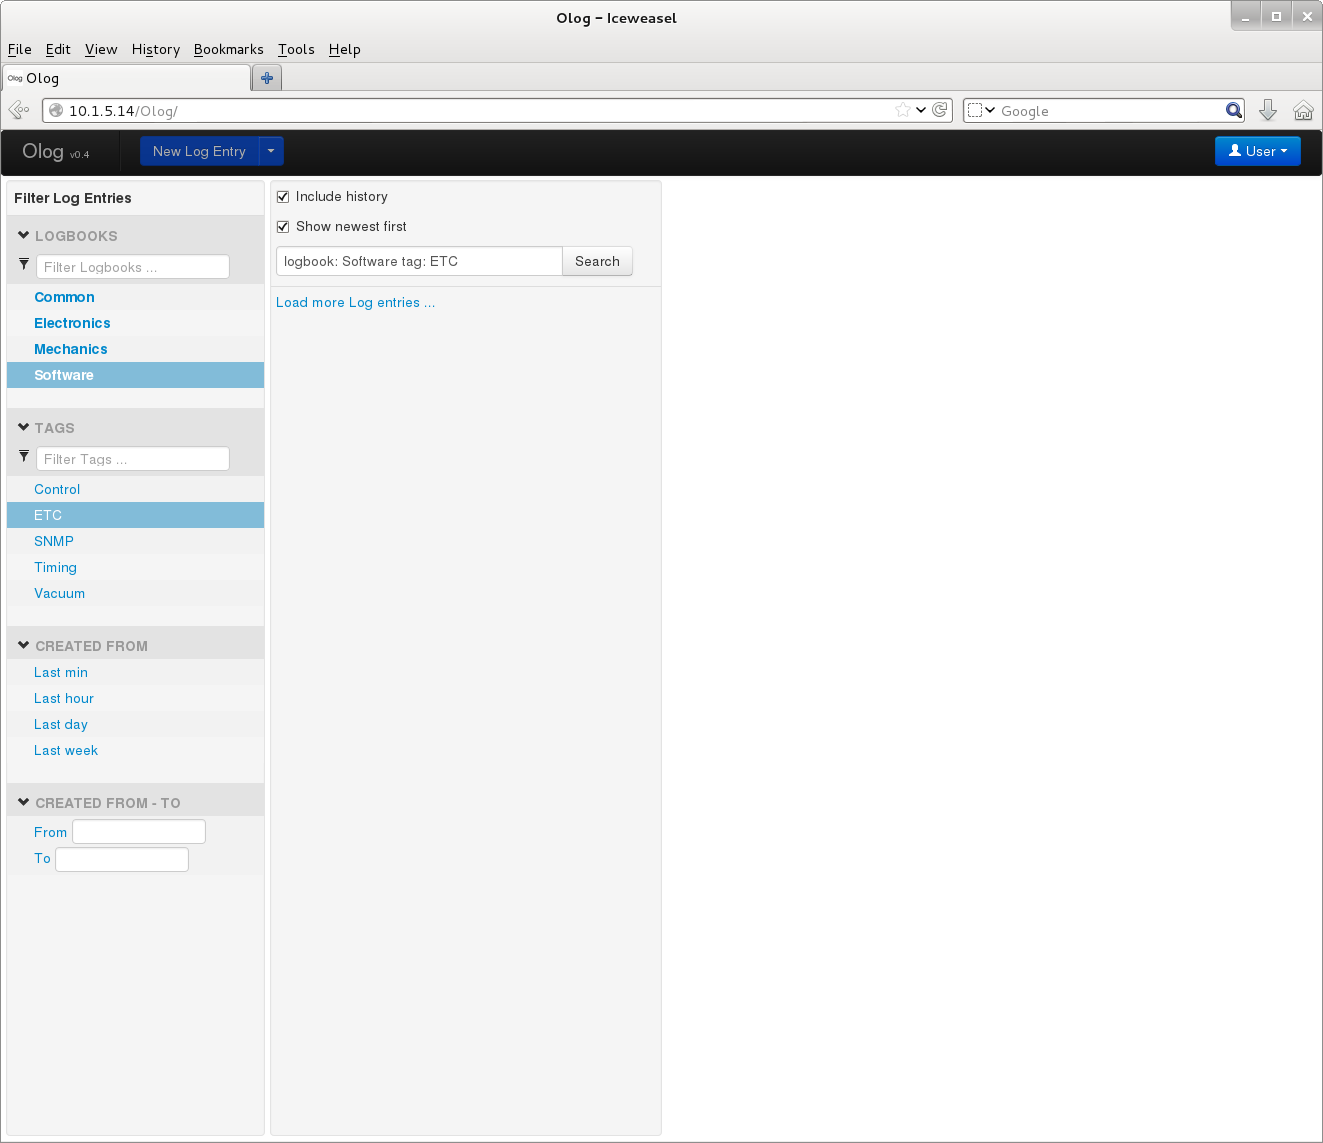
\includegraphics[width=0.96\textwidth]{./images/Web_Client.png}
  \caption{
            Web Client v0.4 beta
          }
  \label{fig:web_client}
\end{figure}

로그 작성을 위해 오른쪽 상단에 있는 User버튼을 눌러 로그인을 한다. 로그인이 완료되면 왼쪽 상단에 있는
New Log Entry 버튼이 활성화 되며 이 버튼을 클릭하여 로그를 작성한다.

\section{CSS Client}
CSS에서 OLog를 사용하기 위해 Edit-Preferences 메뉴에서 아래와 같이 설정한다.
\begin{itemize}
\item Olog Service URL: https://10.1.5.14:8181/Olog/resources
\item use authentication: 체크 해제
\item Prompt User for authentication with each log entry creation: 체크
\item Default logbook: 기본으로 사용할 로그북
\item Page Size: 50
\end{itemize}
설정을 마친 후 CSS 재시작 한다.

로그 작성을 위해 CSS-Utilities-Create Log Entry 메뉴를 선택 한다.
User Name과 Password는 OLog 사용자와 비밀번호를 입력한다.
작성된 로그는 Log Table에서 확인 할 수 있는데
Log Table은 Window-Show View-Other메뉴에서  Other-Log Table을 선택하면 볼 수 있다.
Log Table의 Log Query값에 logbook:Common값을 입력하면 작성된 로그를 확인할 수 있으며,
더블 클릭하면 자세한 내용을 볼 수 있다. 
\begin{figure}[!htb]
  \centering
  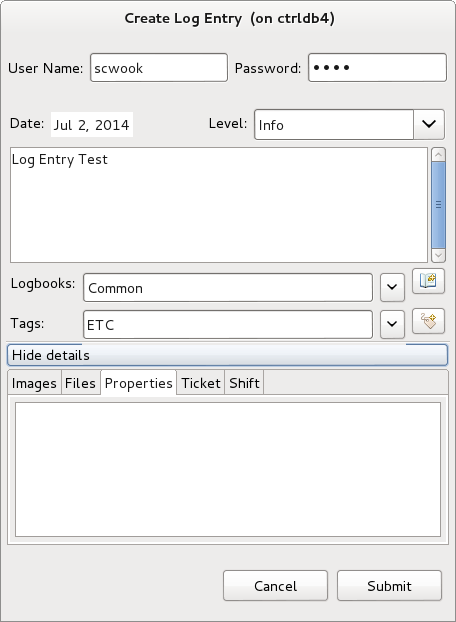
\includegraphics[width=0.45\textwidth]{./images/CSS_Log_Entry.png}
  \caption{
            Create Log Entry
          }
  \label{fig:css_log_entry}
\end{figure}

%\clearpage
\newpage

\bibliographystyle{unsrtnat}

\bibliography{./refs}

\newpage
\appendix
\newappendix
다음 script는 MySQL 데이터 베이스에 OLog DB schema를 생성하는 script이다. 
실제 Table구조(Figure\ref{fig:olog_schema})는 아래 script와 다른 구조로 생성되는데, 
Web Client를 통해 접속하게 되면 최신 DB구조로 변경된다.
예를 들어 levels와 statuses은 삭제되고 entries와 schema\_version이 생성된다.

\begin{lstlisting}[style=termstylenumber, caption={olog\_schema.sql}, label={list:nfsroot-file}]
/*!40101 SET @OLD_CHARACTER_SET_CLIENT=@@CHARACTER_SET_CLIENT */;
/*!40101 SET @OLD_CHARACTER_SET_RESULTS=@@CHARACTER_SET_RESULTS */;
/*!40101 SET @OLD_COLLATION_CONNECTION=@@COLLATION_CONNECTION */;
/*!40101 SET NAMES utf8 */;

/*!40014 SET @OLD_UNIQUE_CHECKS=@@UNIQUE_CHECKS, UNIQUE_CHECKS=0 */;
/*!40014 SET @OLD_FOREIGN_KEY_CHECKS=@@FOREIGN_KEY_CHECKS, FOREIGN_KEY_CHECKS=0 */;
/*!40101 SET @OLD_SQL_MODE=@@SQL_MODE, SQL_MODE='NO_AUTO_VALUE_ON_ZERO' */;

-- Create schema ologdb4
DROP DATABASE IF EXISTS olog;
CREATE DATABASE olog;
USE olog;

-- Definition of table `levels`

DROP TABLE IF EXISTS `levels`;
CREATE TABLE `levels` (
  `id` int(11) NOT NULL AUTO_INCREMENT,
  `name` varchar(200) NOT NULL,
  PRIMARY KEY (`id`),
  UNIQUE KEY `name` (`name`)
) ENGINE=InnoDB AUTO_INCREMENT=6 DEFAULT CHARSET=latin1;

-- Dumping data for table `levels`

/*!40000 ALTER TABLE `levels` DISABLE KEYS */;
INSERT INTO `levels` (`id`,`name`) VALUES
 (1,'Info'),
 (4,'Problem'),
 (3,'Request'),
 (2,'Suggestion'),
 (5,'Urgent');
/*!40000 ALTER TABLE `levels` ENABLE KEYS */;

-- Definition of table `logbooks`

DROP TABLE IF EXISTS `logbooks`;
CREATE TABLE `logbooks` (
  `id` int(11) NOT NULL AUTO_INCREMENT,
  `name` varchar(45) NOT NULL,
  `is_tag` int(1) NOT NULL DEFAULT '0',
  `owner` varchar(45) DEFAULT NULL,
  `status_id` int(11) NOT NULL DEFAULT '1',
  PRIMARY KEY (`id`),
  UNIQUE KEY `name` (`name`),
  KEY `logbooks_status_id_fk` (`status_id`),
  CONSTRAINT `logbooks_status_id_fk` FOREIGN KEY (`status_id`) REFERENCES `statuses` (`id`) ON DELETE NO ACTION ON UPDATE NO ACTION
) ENGINE=InnoDB AUTO_INCREMENT=12 DEFAULT CHARSET=latin1;

-- Dumping data for table `logbooks`

/*!40000 ALTER TABLE `logbooks` DISABLE KEYS */;
INSERT INTO `logbooks` (`id`,`name`,`is_tag`,`owner`,`status_id`) VALUES
 (1,'Operations',0,NULL,1),
 (2,'Electronics Maintenance',0,NULL,1),
 (3,'Mechanical Technicians',0,NULL,1),
 (4,'LOTO',0,NULL,1),
 (5,'Inverpower Power Supplies',1,NULL,1),
 (6,'RF Area',1,NULL,1),
 (7,'Kicker',1,NULL,1),
 (8,'Bumps',1,NULL,1),
 (9,'Septums',1,NULL,1),
 (10,'Large Power Supplies',1,NULL,1),
 (11,'Timing Systems',1,NULL,1);
/*!40000 ALTER TABLE `logbooks` ENABLE KEYS */;

-- Definition of table `logs`

DROP TABLE IF EXISTS `logs`;
CREATE TABLE `logs` (
  `id` int(11) NOT NULL AUTO_INCREMENT,
  `created` timestamp NOT NULL DEFAULT CURRENT_TIMESTAMP,
  `source` varchar(80) NOT NULL DEFAULT '',
  `owner` varchar(32) NOT NULL,
  `level_id` int(11) NOT NULL DEFAULT '1',
  `status_id` int(11) NOT NULL DEFAULT '1',
  `description` mediumtext NOT NULL,
  `md5entry` varchar(32) NOT NULL DEFAULT '',
  `md5recent` mediumtext NOT NULL,
  `parent_id` int(11) DEFAULT NULL,
  PRIMARY KEY (`id`),
  KEY `level_id_fk` (`level_id`),
  KEY `log_parent_id_fk` (`parent_id`),
  KEY `status_id_fk` (`status_id`),
  CONSTRAINT `level_id_fk` FOREIGN KEY (`level_id`) REFERENCES `levels` (`id`) ON DELETE NO ACTION ON UPDATE NO ACTION,
  CONSTRAINT `log_parent_id_fk` FOREIGN KEY (`parent_id`) REFERENCES `logs` (`id`) ON DELETE NO ACTION ON UPDATE NO ACTION,
  CONSTRAINT `status_id_fk` FOREIGN KEY (`status_id`) REFERENCES `statuses` (`id`) ON DELETE NO ACTION ON UPDATE NO ACTION
) ENGINE=InnoDB AUTO_INCREMENT=1 DEFAULT CHARSET=latin1;

-- Definition of table `logs_logbooks`

DROP TABLE IF EXISTS `logs_logbooks`;
CREATE TABLE `logs_logbooks` (
  `id` int(11) NOT NULL AUTO_INCREMENT,
  `log_id` int(11) NOT NULL,
  `logbook_id` int(11) NOT NULL,
  `state` enum('open','closed') DEFAULT NULL,
  `created` timestamp NOT NULL DEFAULT CURRENT_TIMESTAMP,
  `status_id` int(11) NOT NULL DEFAULT '1',
  PRIMARY KEY (`id`),
  KEY `log_id_fk` (`log_id`),
  KEY `logbook_id_fk` (`logbook_id`) USING BTREE,
  KEY `logs_logbooks_status_id_fk` (`status_id`),
  CONSTRAINT `logs_logbooks_status_id_fk` FOREIGN KEY (`status_id`) REFERENCES `statuses` (`id`) ON DELETE NO ACTION ON UPDATE NO ACTION,
  CONSTRAINT `logs_logbooks_logbook_id_fk` FOREIGN KEY (`logbook_id`) REFERENCES `logbooks` (`id`) ON DELETE NO ACTION ON UPDATE NO ACTION,
  CONSTRAINT `logs_logbooks_log_id_fk` FOREIGN KEY (`log_id`) REFERENCES `logs` (`id`) ON DELETE NO ACTION ON UPDATE NO ACTION
) ENGINE=InnoDB AUTO_INCREMENT=1 DEFAULT CHARSET=latin1;

-- Definition of table `properties`

DROP TABLE IF EXISTS `properties`;
CREATE TABLE  `properties` (
  `id` int(11) NOT NULL AUTO_INCREMENT,
  `name` varchar(200) NOT NULL,
  `status_id` tinyint(1) NOT NULL,
  PRIMARY KEY (`id`)
) ENGINE=InnoDB AUTO_INCREMENT=4 DEFAULT CHARSET=latin1;

-- Dumping data for table `properties`

/*!40000 ALTER TABLE `properties` DISABLE KEYS */;
/*!40000 ALTER TABLE `properties` ENABLE KEYS */;

-- Definition of table `attributes`

DROP TABLE IF EXISTS `attributes`;
CREATE TABLE  `attributes` (
  `id` int(11) NOT NULL AUTO_INCREMENT,
  `property_id` int(11) NOT NULL,
  `name` varchar(200) NOT NULL,
  `status_id` tinyint(1) NOT NULL,
  PRIMARY KEY (`id`),
  KEY `attributes_property_id_fk` (`property_id`),
  CONSTRAINT `attributes_property_id_fk` FOREIGN KEY (`property_id`) REFERENCES `properties` (`id`) ON DELETE NO ACTION ON UPDATE NO ACTION
) ENGINE=InnoDB AUTO_INCREMENT=19 DEFAULT CHARSET=latin1;

-- Definition of table `logs_attributes`

DROP TABLE IF EXISTS `logs_attributes`;
CREATE TABLE  `logs_attributes` (
  `id` int(11) NOT NULL AUTO_INCREMENT,
  `log_id` int(11) NOT NULL,
  `attribute_id` int(11) NOT NULL,
  `value` varchar(200) NOT NULL,
  `grouping_num` int(11) NOT NULL,
  PRIMARY KEY (`id`),
  KEY `logs_attributes_attribute_id_fk` (`attribute_id`),
  KEY `logs_attributes_log_id_fk` (`log_id`),
  CONSTRAINT `logs_attributes_attribute_id_fk` FOREIGN KEY (`attribute_id`) REFERENCES `attributes` (`id`) ON DELETE NO ACTION ON UPDATE NO ACTION,
  CONSTRAINT `logs_attributes_log_id_fk` FOREIGN KEY (`log_id`) REFERENCES `logs` (`id`) ON DELETE NO ACTION ON UPDATE NO ACTION
) ENGINE=InnoDB AUTO_INCREMENT=179 DEFAULT CHARSET=latin1;

-- Definition of table `statuses`

DROP TABLE IF EXISTS `statuses`;
CREATE TABLE `statuses` (
  `id` int(11) NOT NULL AUTO_INCREMENT,
  `name` varchar(45) NOT NULL,
  PRIMARY KEY (`id`)
) ENGINE=InnoDB AUTO_INCREMENT=3 DEFAULT CHARSET=latin1;

-- Dumping data for table `statuses`

/*!40000 ALTER TABLE `statuses` DISABLE KEYS */;
INSERT INTO `statuses` (`id`,`name`) VALUES
 (1,'Active'),
 (2,'Inactive');
/*!40000 ALTER TABLE `statuses` ENABLE KEYS */;

-- Definition of table `subscriptions`

DROP TABLE IF EXISTS `subscriptions`;
CREATE TABLE `subscriptions` (
  `id` int(11) NOT NULL AUTO_INCREMENT,
  `tag_id` int(11) NOT NULL,
  `email` varchar(250) NOT NULL DEFAULT '',
  `webhook` varchar(250) DEFAULT NULL,
  `level_id` int(11) NOT NULL,
  PRIMARY KEY (`id`),
  KEY `subscriptions_tag_id_fk` (`tag_id`),
  CONSTRAINT `subscriptions_tag_id_fk` FOREIGN KEY (`tag_id`) REFERENCES `logbooks` (`id`) ON DELETE NO ACTION ON UPDATE NO ACTION
) ENGINE=InnoDB DEFAULT CHARSET=latin1;

-- Dumping data for table `subscriptions`

/*!40000 ALTER TABLE `subscriptions` DISABLE KEYS */;
/*!40000 ALTER TABLE `subscriptions` ENABLE KEYS */;

/*!40101 SET SQL_MODE=@OLD_SQL_MODE */;
/*!40014 SET FOREIGN_KEY_CHECKS=@OLD_FOREIGN_KEY_CHECKS */;
/*!40014 SET UNIQUE_CHECKS=@OLD_UNIQUE_CHECKS */;
/*!40101 SET CHARACTER_SET_CLIENT=@OLD_CHARACTER_SET_CLIENT */;
/*!40101 SET CHARACTER_SET_RESULTS=@OLD_CHARACTER_SET_RESULTS */;
/*!40101 SET COLLATION_CONNECTION=@OLD_COLLATION_CONNECTION */;
/*!40101 SET CHARACTER_SET_CLIENT=@OLD_CHARACTER_SET_CLIENT */;
\end{lstlisting}

\newpage
\newappendix
LDAP 사용이 어려운 경우 다음과 같이 File Realm을 사용할 수 있다\\
Configurations - server-config - Security - Realms에서 새로운 Realms을 생성 후
아래와 같이 설정한다.
\begin{itemize}
\item Name: olog
\item Class Name: com.sun.enterprise.security.auth.realm.file.FileRealm
\item JAAS Context: fileRealm
\item Key File: \$\{com.sun.aas.instanceRoot\}/config/olog\_keyfile 
\end{itemize}
저장 후 방금 생성한 olog를 선택하면 왼쪽 상단에 있는 Manage Users를 클릭하여 
사용자를 추가한다. Group List는 관리자 권한의 경우 olog-admins를 일반 사용자의
경우 olog-logs를 입력하면 된다.

\end{document}
